\documentclass{article}
\usepackage{tikz}
\usetikzlibrary{matrix,chains,positioning,decorations.pathreplacing,arrows}
\usepackage{mathtools}


\begin{document}
\section{Exercise \textit{(Perceptron (6p))}}
\begin{itemize}
	\item [1.] Sketch a single neuron perceptron with weights and threshold $\theta$ for the following logical
functions: Our network is set up like this:\\
	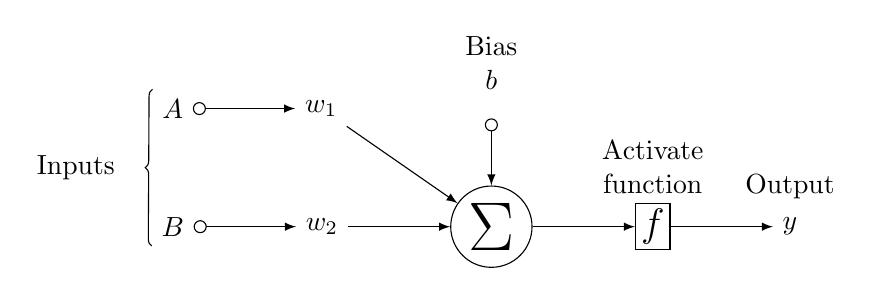
\begin{tikzpicture}[
init/.style={
  draw,
  circle,
  inner sep=2pt,
  font=\Huge,
  join = by -latex
},
squa/.style={
  draw,
  inner sep=2pt,
  font=\Large,
  join = by -latex
},
start chain=2,node distance=13mm
]
\node[on chain=2] 
  (x2) {$B$};
\node[on chain=2,join=by o-latex] 
  {$w_2$};
\node[on chain=2,init] (sigma) 
  {$\displaystyle\Sigma$};
\node[on chain=2,squa,label=above:{\parbox{2cm}{\centering Activate \\ function}}]   
  {$f$};
\node[on chain=2,label=above:Output,join=by -latex] 
  {$y$};
\begin{scope}[start chain=1]
\node[on chain=1] at (0,1.5cm) 
  (x1) {$A$};
\node[on chain=1,join=by o-latex] 
  (w1) {$w_1$};
\end{scope}

\node[label=above:\parbox{2cm}{\centering Bias \\ $b$}] at (sigma|-w1) (b) {};

\draw[-latex] (w1) -- (sigma);
\draw[o-latex] (b) -- (sigma);

\draw[decorate,decoration={brace,mirror}] (x1.north west) -- node[left=10pt] {Inputs} (x2.south west);
\end{tikzpicture} \\
We assume $A,B \in \{-1 , 1\}$
	\item [(a)] $(A\wedge B)\vee(\neg A \wedge B)$ \\
		$\leftrightarrow$\footnote{since B is either 1 or 0} \\
		$B$ \\
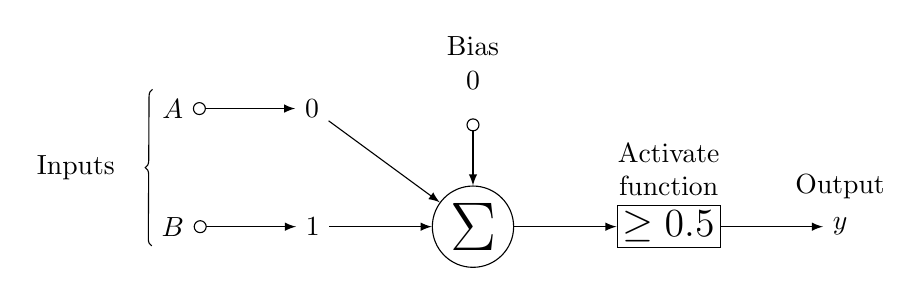
\begin{tikzpicture}[
init/.style={
  draw,
  circle,
  inner sep=2pt,
  font=\Huge,
  join = by -latex
},
squa/.style={
  draw,
  inner sep=2pt,
  font=\Large,
  join = by -latex
},
start chain=2,node distance=13mm
]
\node[on chain=2] 
  (x2) {$B$};
\node[on chain=2,join=by o-latex] 
  {$1$};
\node[on chain=2,init] (sigma) 
  {$\displaystyle\Sigma$};
\node[on chain=2,squa,label=above:{\parbox{2cm}{\centering Activate \\ function}}]   
  {$\geq 0.5$};
\node[on chain=2,label=above:Output,join=by -latex] 
  {$y$};
\begin{scope}[start chain=1]
\node[on chain=1] at (0,1.5cm) 
  (x1) {$A$};
\node[on chain=1,join=by o-latex] 
  (w1) {$0$};
\end{scope}

\node[label=above:\parbox{2cm}{\centering Bias \\ $0$}] at (sigma|-w1) (b) {};

\draw[-latex] (w1) -- (sigma);
\draw[o-latex] (b) -- (sigma);

\draw[decorate,decoration={brace,mirror}] (x1.north west) -- node[left=10pt] {Inputs} (x2.south west);
\end{tikzpicture}
\item [(b)] $(A \wedge B) \vee (\neg A \wedge B) \vee (A \wedge \neg B)$ \\
	$\leftrightarrow$\footnote{again, bracketing out $B$ and $\neg B$ and $A$ and $\neg A$ } \\
	$A \vee B$\\
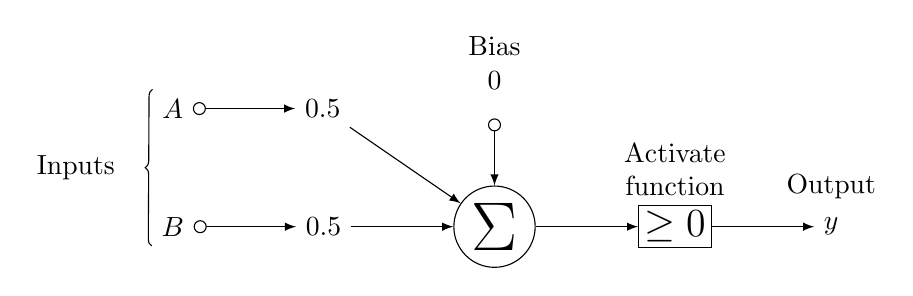
\begin{tikzpicture}[
init/.style={
  draw,
  circle,
  inner sep=2pt,
  font=\Huge,
  join = by -latex
},
squa/.style={
  draw,
  inner sep=2pt,
  font=\Large,
  join = by -latex
},
start chain=2,node distance=13mm
]
\node[on chain=2] 
  (x2) {$B$};
\node[on chain=2,join=by o-latex] 
  {$0.5$};
\node[on chain=2,init] (sigma) 
  {$\displaystyle\Sigma$};
\node[on chain=2,squa,label=above:{\parbox{2cm}{\centering Activate \\ function}}]   
  {$\geq 0$};
\node[on chain=2,label=above:Output,join=by -latex] 
  {$y$};
\begin{scope}[start chain=1]
\node[on chain=1] at (0,1.5cm) 
  (x1) {$A$};
\node[on chain=1,join=by o-latex] 
  (w1) {$0.5$};
\end{scope}

\node[label=above:\parbox{2cm}{\centering Bias \\ $0$}] at (sigma|-w1) (b) {};

\draw[-latex] (w1) -- (sigma);
\draw[o-latex] (b) -- (sigma);

\draw[decorate,decoration={brace,mirror}] (x1.north west) -- node[left=10pt] {Inputs} (x2.south west);
\end{tikzpicture}
\end{itemize} \newpage
\begin{itemize}
	\item [2.] Draw pictures similar to slide page 36 in chapter 7 for the boolean functions below, and
give weights for the perceptron or argue if no such weight exist. The features $x_1, x_2$ and
output $y$ can only take values -1 or +1.
\end{itemize}

 \[ y =  \begin{dcases} 
    						  +1 : x_1 = 1 , x_2 = -1 \\
					          -1 : otherwise
					   \end{dcases}
					   \] \\
$\to w_1 = 1 , w_2 = -1 , b = - 1 , f(x) = 1 \leftrightarrow x \geq 0.5$					   
					
%\begin{figure}
	\includegraphics[scale = 0.4]{untitled}	
%\end{figure}
\section{Exercise \textit{(Perceptron (6p))}}
Simple classification problem for single neuron perceptron.
\begin{itemize}
	\item [1.] Draw a decision boundary in figure 2 (a) and (b) and find weights and bias for each network. \\
\end{itemize}
	%\begin{figure}
	\includegraphics[scale = 0.4]{dots}	 \\
	%\end{figure}
	\begin{itemize}
		\item [(a)] $\vec{w} = (-1 ,\frac{1}{2}) , b = 0$ (b) $\vec{w} = (-1 , \frac{3}{2}) , b = -2$
	\end{itemize}
\begin{itemize}
	\item [2.] Determine the margin of the the separation line for each figure. (Hint: Compute the
distance between each point in the figure to the selected decision boundary)
\end{itemize}
\color{black}
\footnotesize
    \begin{verbatim}
close all % plotting the data and calculating the point line distance by 
hold on % projecting the points onto the unit normal vector
points = [-2,-2,-2,0,0,2,2,2 ; -2,0,2,-2,2,-2,0,2];
scatter(points(1,:),points(2,:),[],[0,0,0,10,0,10,10,10])
normal = [-1,0.5];
normal = normal * (1./sqrt(normal*normal.'));
quiver(0,0,normal(1),normal(2))
xlim([-2.5 2.5])
ylim([-2.5 2.5])

distances = abs(normal * points);
margin = min(distances)
___________________________
margin =

    0.8944
___________________________

close all;
hold on;
points2 = [0,0,1,2 ; -1,-3,0,-2];
scatter(points2(1,:),points2(2,:),[],[0,10,0,10])

xlim([-4 4])
ylim([-4 4])

normal2 = [-1,1.5];
normal2 = normal2 * (1./sqrt(normal2*normal2.'));

quiver(0,-2,normal2(1),normal2(2))
distances2 = abs(normal2 * [points2(1,:) ; points2(2,:) - 2]);

margin2 = min(distances2)

___________________________

margin2 =

    2.2188
___________________________

\end{verbatim}
\normalsize
\newpage
\end{document}